In this chapter the results from the experiments will be shown and analyzed. First off, the model will be discussed without any policies in effect. Then, the results will be discussed and briefly analysed per policy or policy lever . 

\iffalse
1.	Show and explain results without policies
2.	Show and explain consequences of scenarios for model behaviour
3.	Show and explain consequences of policies for each scenario (i.e., robustness) 
\fi
\subsection{Results of the model without policies}

The model was first run without any policies in place to study the effects of the scenarios on the situation as is. 

\subsubsection{Base}
\label{s:b_base}
The model was run without any scenarios to generate behaviour, dubbed the base run. The behaviour of the KPIs was studied for this base behaviour.

\begin{figure}[h!]
    \centering
    \begin{minipage}{0.45\textwidth}
        \centering
        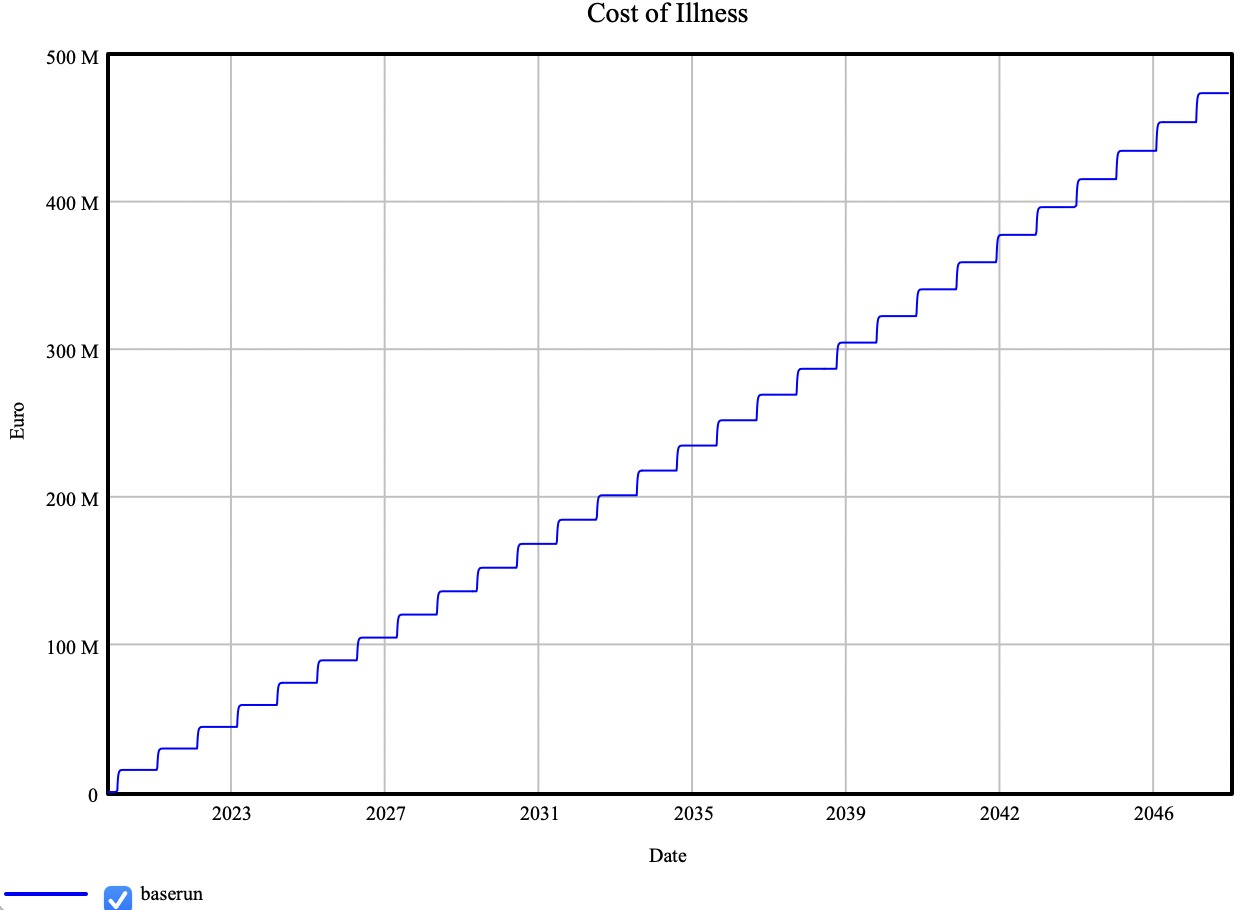
\includegraphics[width=1\textwidth]{images/base_COI.jpeg} % first figure itself
        \caption{Cost of Illness in the base run}
        \label{fig:b_coi}
    \end{minipage}\hfill
    \begin{minipage}{0.45\textwidth}
        \centering
        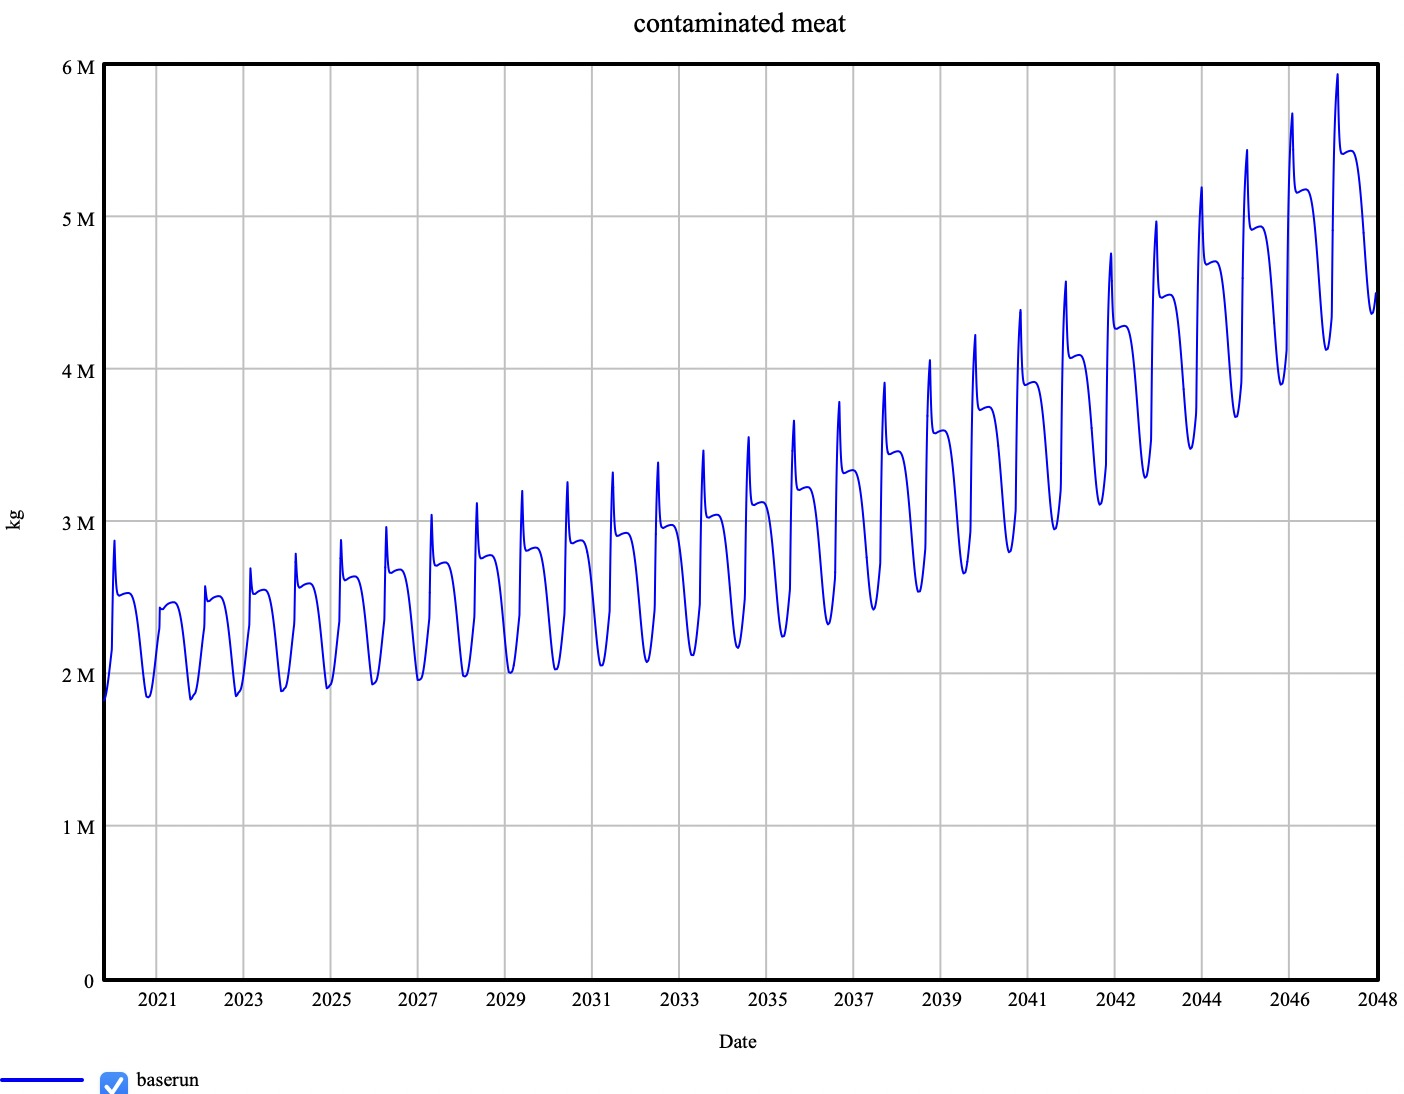
\includegraphics[width=1\textwidth]{images/base_meat.jpeg} % second figure itself
        \caption{Contaminated chicken meat in the base run}
        \label{fig:b_meat}
    \end{minipage}
\end{figure}

\begin{figure}[h!]
    \centering
    \begin{minipage}{0.45\textwidth}
        \centering
        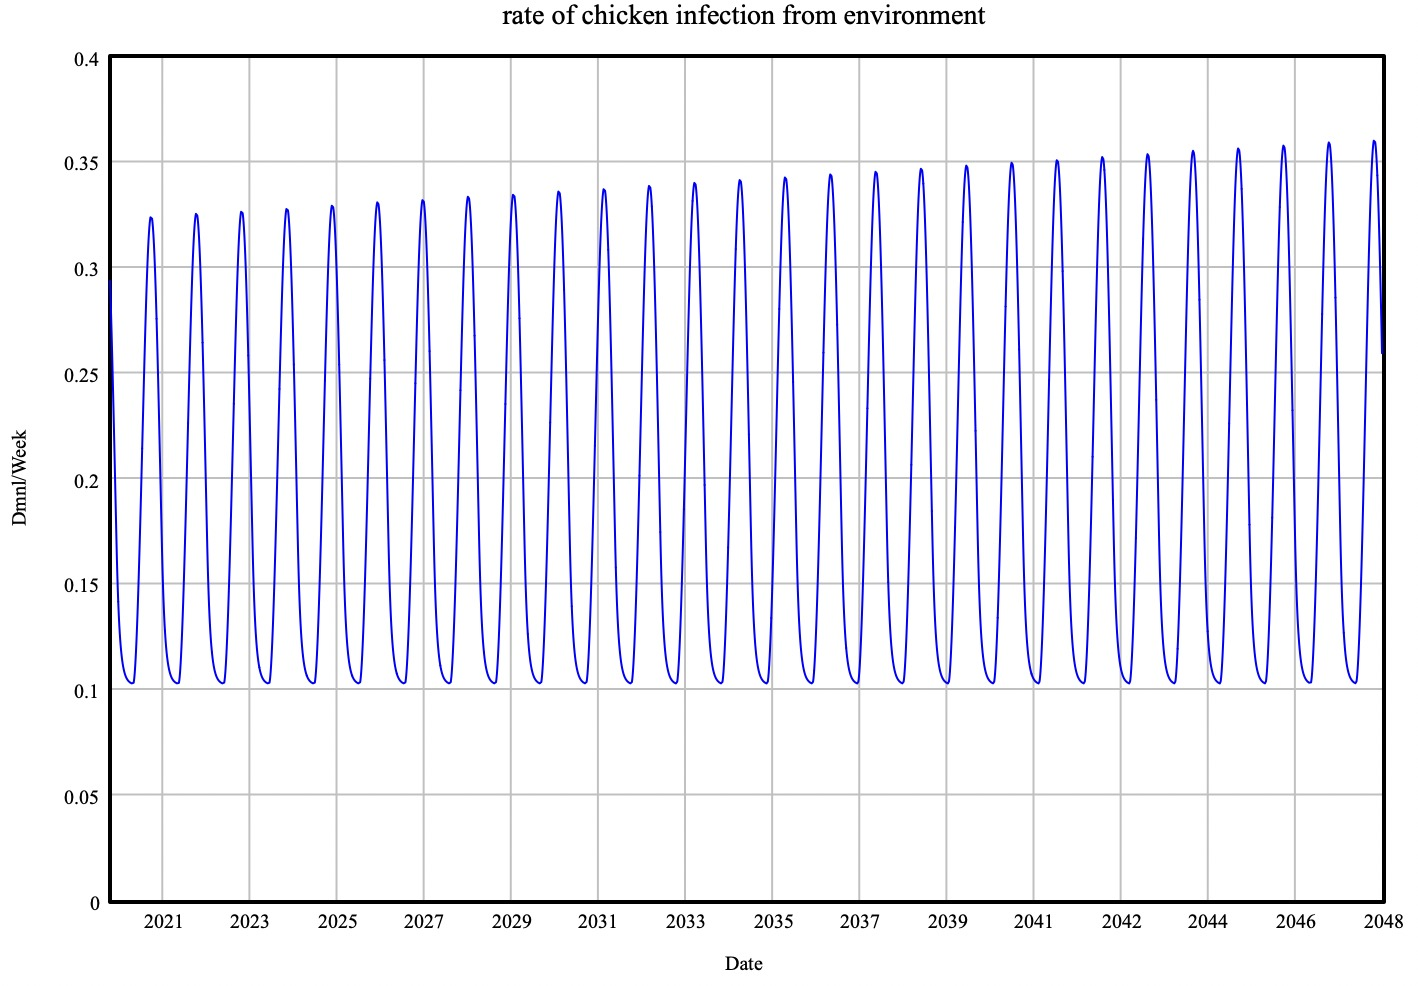
\includegraphics[width=1\textwidth]{images/base_chicken.jpeg} 
        \caption{Chicken infections from environment in the base run}
        \label{fig:b_chicken}
    \end{minipage}\hfill
    \begin{minipage}{0.45\textwidth}
        \centering
        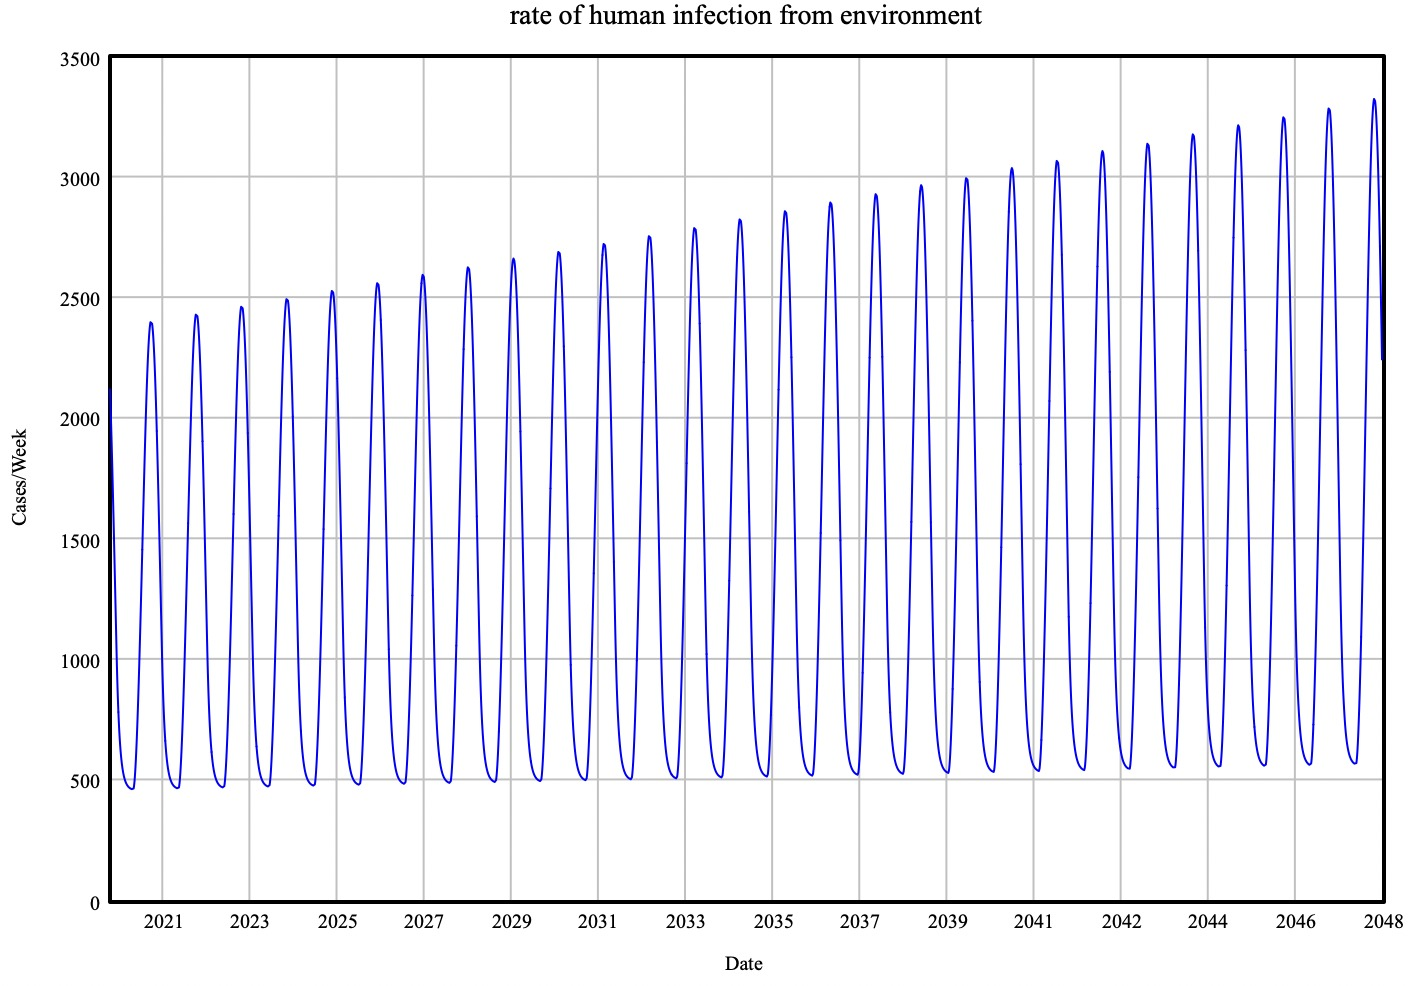
\includegraphics[width=1\textwidth]{images/base_human.jpeg}
        \caption{Human infections from environment in the base run}
        \label{fig:b_human}
    \end{minipage}
\end{figure}

The model generated behaviour that was generally consistent with the dynamic hypothesis, with three main exceptions:

The contaminated meat stock (Figure \ref{fig:b_meat}) exhibits unusual behaviour due to a structural uncertainty linking the number of \textit{campylobacter} cases to changes in meat consumption. After a given threshold number of cases have occurred in the population, we assume there would be a change in behaviour of people choosing to consume less chicken meat to avoid infections, this results in a temporary spike in the contaminated meat stock while the poultry industry responds to changing consumer demand.

Secondly, we did not account for seasonality in the development of the contaminated meat stock. It had been conceptualised in the aggregate sense, leaving the seasonality out of it. 

The model produces a stair-like graph for the cost of illness, where we had hypothesized a straight line instead. This has to with the switch in units mentioned in section \ref{s:verification}, where the model goes from weeks to years. This means that the increase in Cost of Illness occurs once every 52 weeks and then remains the same for the rest of the year, resulting in the stairs we can see in (Figure \ref{fig:b_coi}). Should the time step of the model have been consistent, it would have resulted in a straight line as hypothesized. 
\subsection{Consequences of scenarios for model behaviour}
\subsubsection{Population scenarios}

\begin{figure}[h!]
    \centering
    \begin{minipage}{0.45\textwidth}
        \centering
        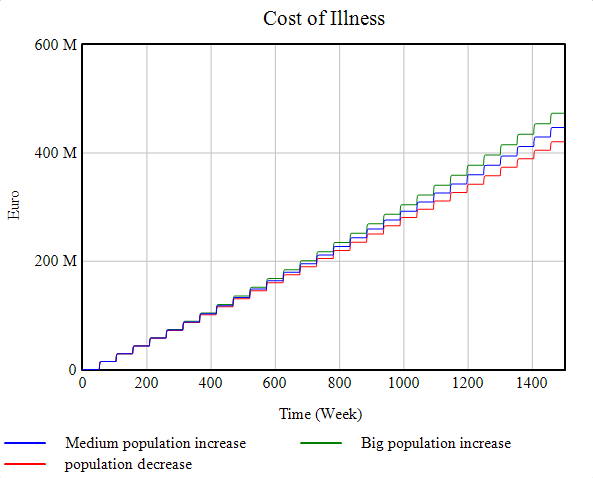
\includegraphics[width=1\textwidth]{images/sensitivity/Population COI.png} % first figure itself
        \caption{Cost of Illness in the different population scenarios}
        \label{fig:pop_coi}
    \end{minipage}\hfill
    \begin{minipage}{0.45\textwidth}
        \centering
        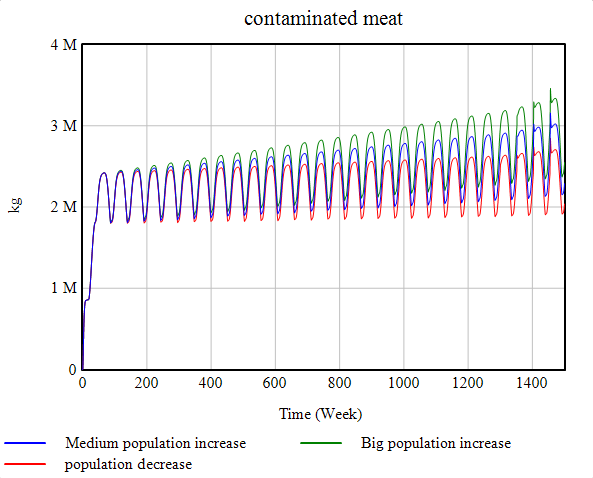
\includegraphics[width=1\textwidth]{images/sensitivity/Population contaminated meat.png} % second figure itself
        \caption{Contaminated chicken meat in the different population scenarios}
        \label{fig:pop_meat}
    \end{minipage}
\end{figure}

\begin{figure}[h!]
    \centering
    \begin{minipage}{0.45\textwidth}
        \centering
        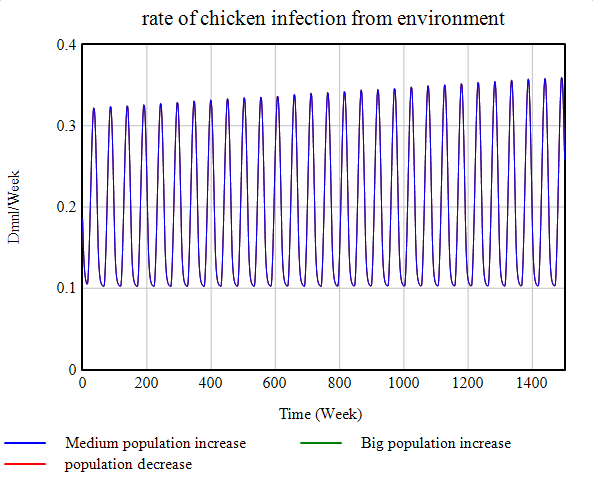
\includegraphics[width=1\textwidth]{images/sensitivity/Population chicken infection.png} 
        \caption{Chicken infections from environment in the different population scenarios}
        \label{fig:pop_chicken}
    \end{minipage}\hfill
    \begin{minipage}{0.45\textwidth}
        \centering
        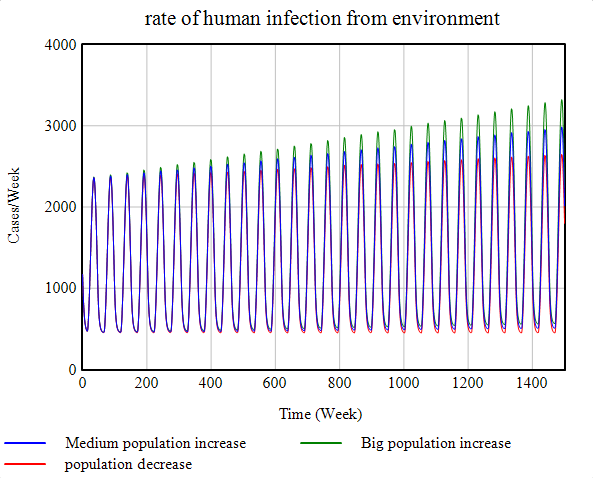
\includegraphics[width=1\textwidth]{images/sensitivity/Population human infection.png}
        \caption{Human infections from environment in the different population scenarios}
        \label{fig:pop_human}
    \end{minipage}
\end{figure}

\subsubsection{Climate scenarios}

\textbf{Average temperature increase}

\begin{figure}[h!]
    \centering
    \begin{minipage}{0.45\textwidth}
        \centering
        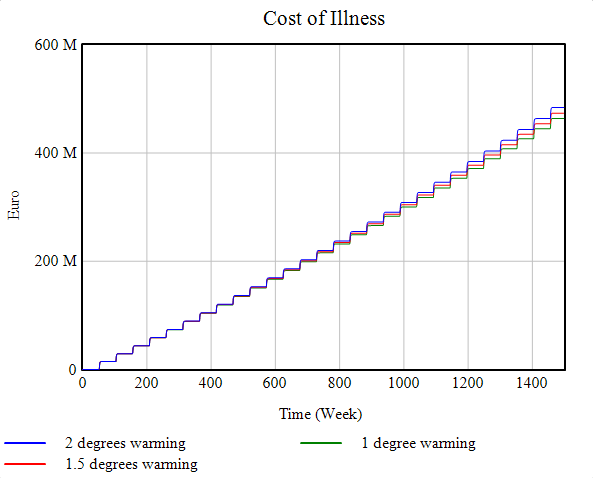
\includegraphics[width=1\textwidth]{images/sensitivity/Temperature projection COI.png} % first figure itself
        \caption{Cost of Illness in the different temperature increase scenarios}
        \label{fig:temp_coi}
    \end{minipage}\hfill
    \begin{minipage}{0.45\textwidth}
        \centering
        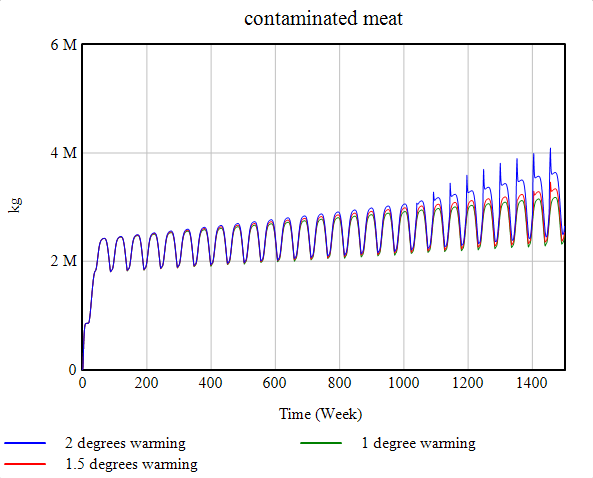
\includegraphics[width=1\textwidth]{images/sensitivity/Temperature projection contaminated meat.png} % second figure itself
        \caption{Contaminated chicken meat in the different temperature increase scenarios}
        \label{fig:temp_meat}
    \end{minipage}
\end{figure}

\begin{figure}[h!]
    \centering
    \begin{minipage}{0.45\textwidth}
        \centering
        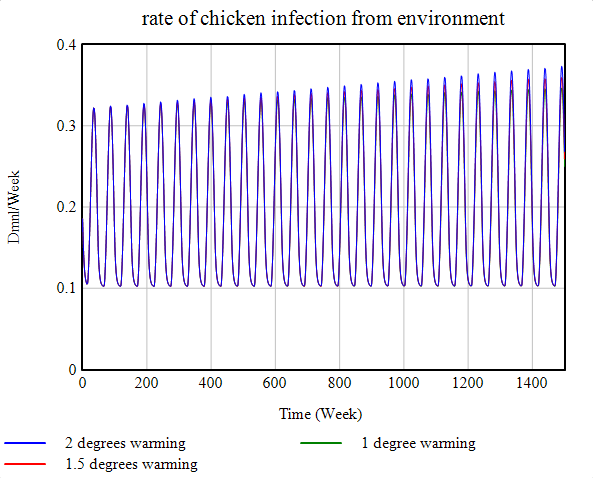
\includegraphics[width=1\textwidth]{images/sensitivity/Temperature projection chicken infection.png} 
        \caption{Chicken infections from environment in the different temperature increase scenarios}
        \label{fig:temp_chicken}
    \end{minipage}\hfill
    \begin{minipage}{0.45\textwidth}
        \centering
        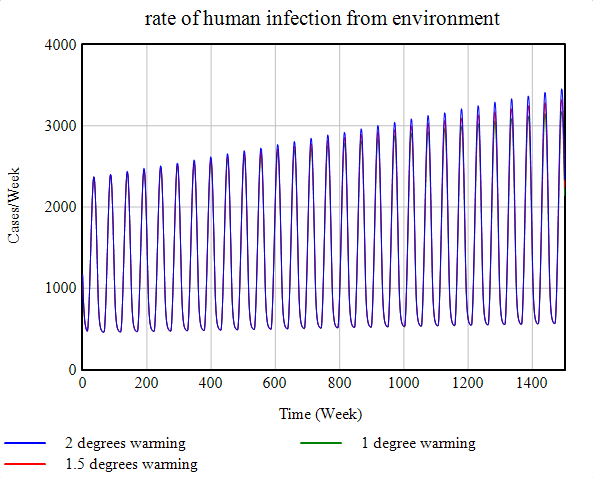
\includegraphics[width=1\textwidth]{images/sensitivity/Temperature projection human infection.png}
        \caption{Human infections from environment in the different temperature increase scenarios}
        \label{fig:temp_human}
    \end{minipage}
\end{figure}

\textbf{Seasonal temperature increase}

\begin{figure}[h!]
    \centering
    \begin{minipage}{0.45\textwidth}
        \centering
        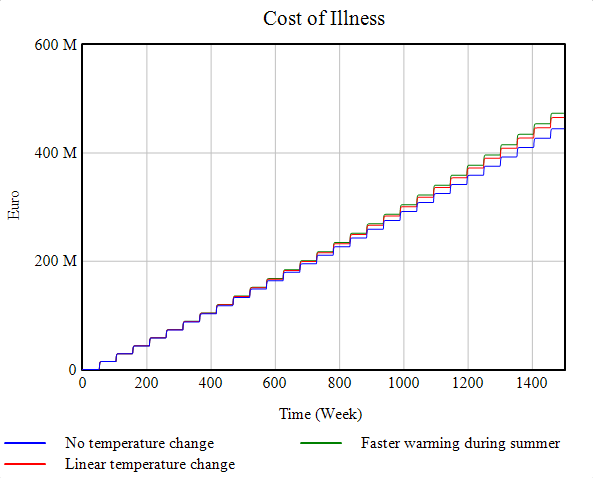
\includegraphics[width=1\textwidth]{images/sensitivity/Seasonal temperature COI.png} % first figure itself
        \caption{Cost of Illness in the different temperature seasonality scenarios}
        \label{fig:season_coi}
    \end{minipage}\hfill
    \begin{minipage}{0.45\textwidth}
        \centering
        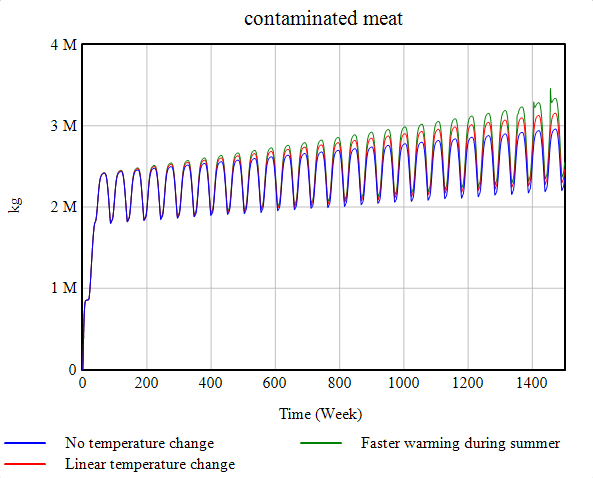
\includegraphics[width=1\textwidth]{images/sensitivity/Seasonal temperature contaminated meat.png} % second figure itself
        \caption{Contaminated chicken meat in the different temperature seasonality scenarios}
        \label{fig:season_meat}
    \end{minipage}
\end{figure}

\begin{figure}[h!]
    \centering
    \begin{minipage}{0.45\textwidth}
        \centering
        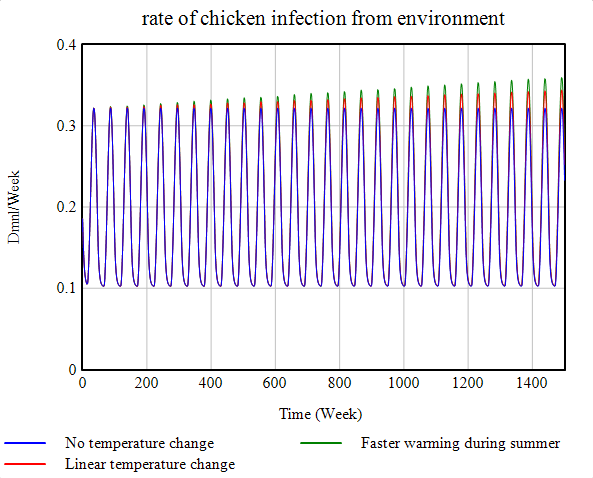
\includegraphics[width=1\textwidth]{images/sensitivity/Seasonal temperature chicken infection.png} 
        \caption{Chicken infections from environment in the different temperature seasonality scenarios}
        \label{fig:season_chicken}
    \end{minipage}\hfill
    \begin{minipage}{0.45\textwidth}
        \centering
        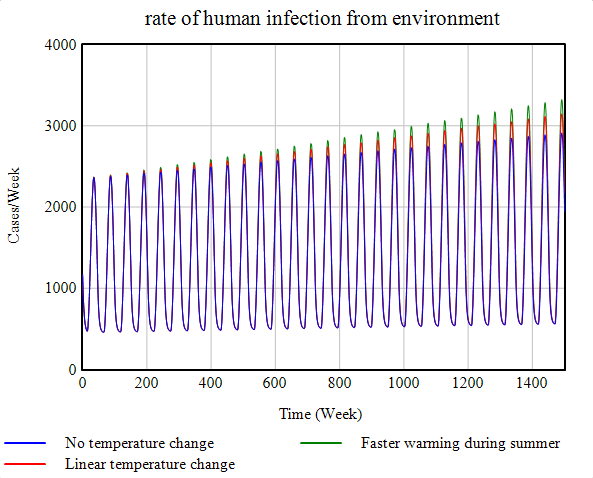
\includegraphics[width=1\textwidth]{images/sensitivity/Seasonal temperature human infection.png}
        \caption{Human infections from environment in the different temperature seasonality scenarios}
        \label{fig:season_human}
    \end{minipage}
\end{figure}

\subsubsection{Public health scenarios}

\begin{figure}[h!]
    \centering
    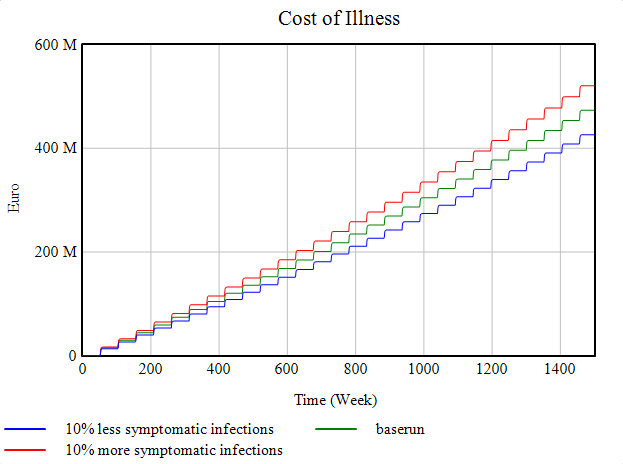
\includegraphics[width=1\textwidth]{images/sensitivity/Symptomatic COI.png} 
    \caption{Cost of illness in the different symptomatic infection scenarios}
    \label{fig:symptom_COI}
\end{figure}

\subsubsection{Multivariate sensitivity analysis}



\subsection{Consequences of policies under scenarios}
\subsubsection{Base model}

A policy regarding slaughtering was modeled into the base model, which will be tested under the same scenarios as the base model. The food safety and handling policy, also dubbed the Safe Slaughtering policy, goes into effect when Cost of Illness reaches a certain threshold, set at a 100 million euros. This policy means that the rate of cross-contamination drops by 20\%.  

\begin{figure}[h!]
    \centering
    \begin{minipage}{0.45\textwidth}
        \centering
        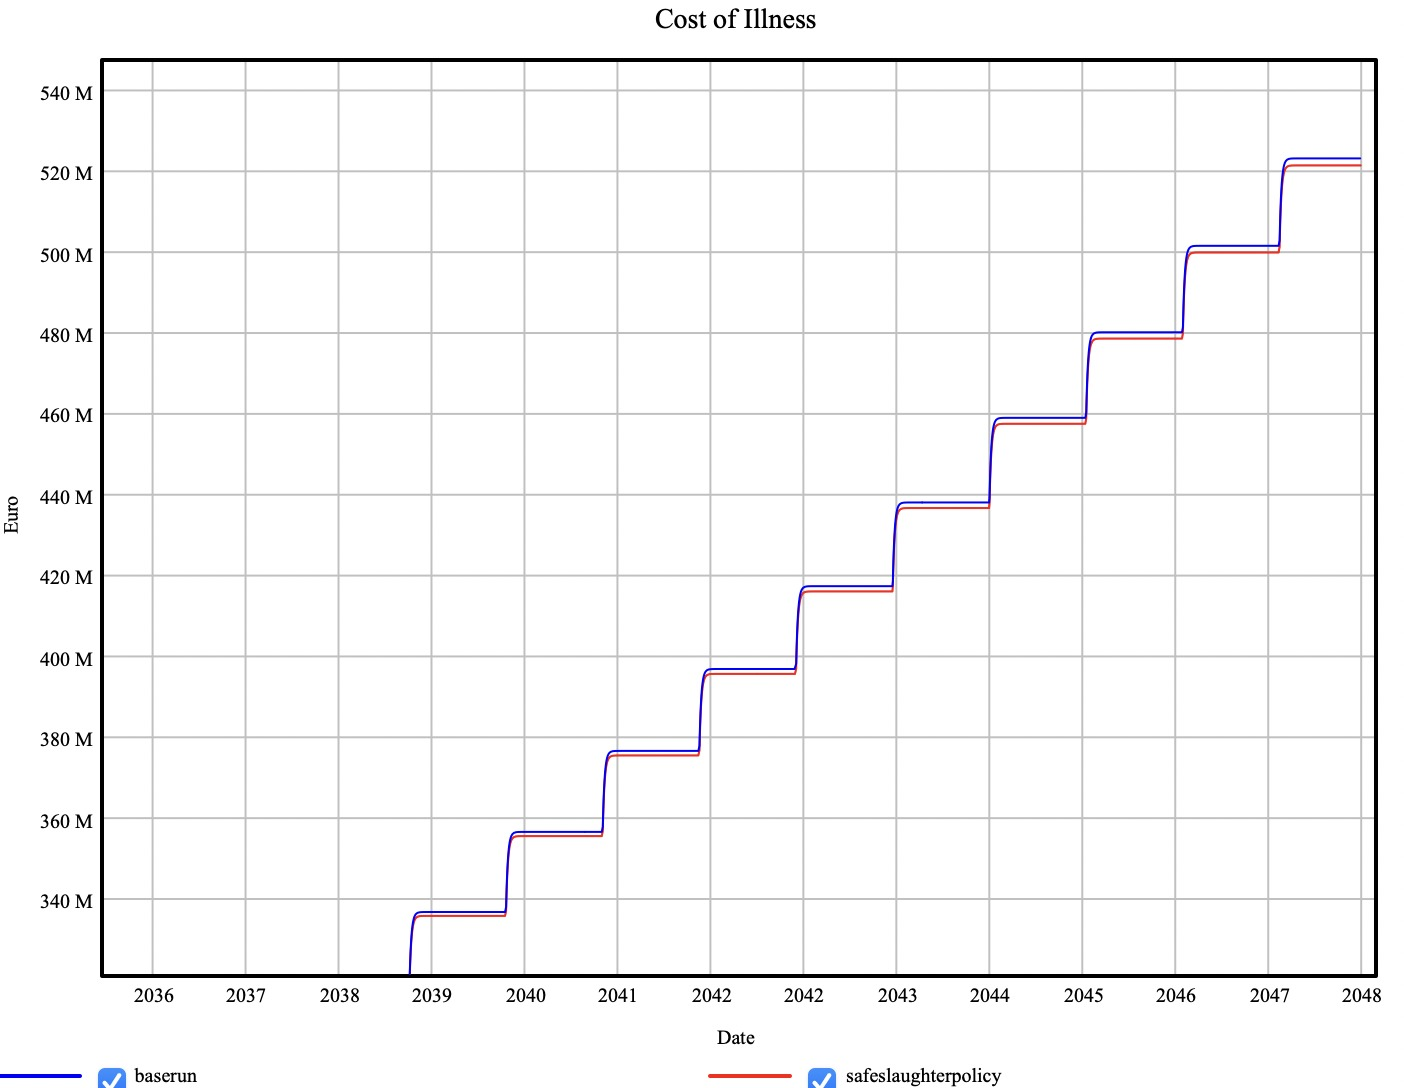
\includegraphics[width=1\textwidth]{images/p_coi.jpeg} 
        \caption{Cost of Illness in the Safe Slaughtering base run}
        \label{fig:p_coi}
    \end{minipage}\hfill
    \begin{minipage}{0.45\textwidth}
        \centering
        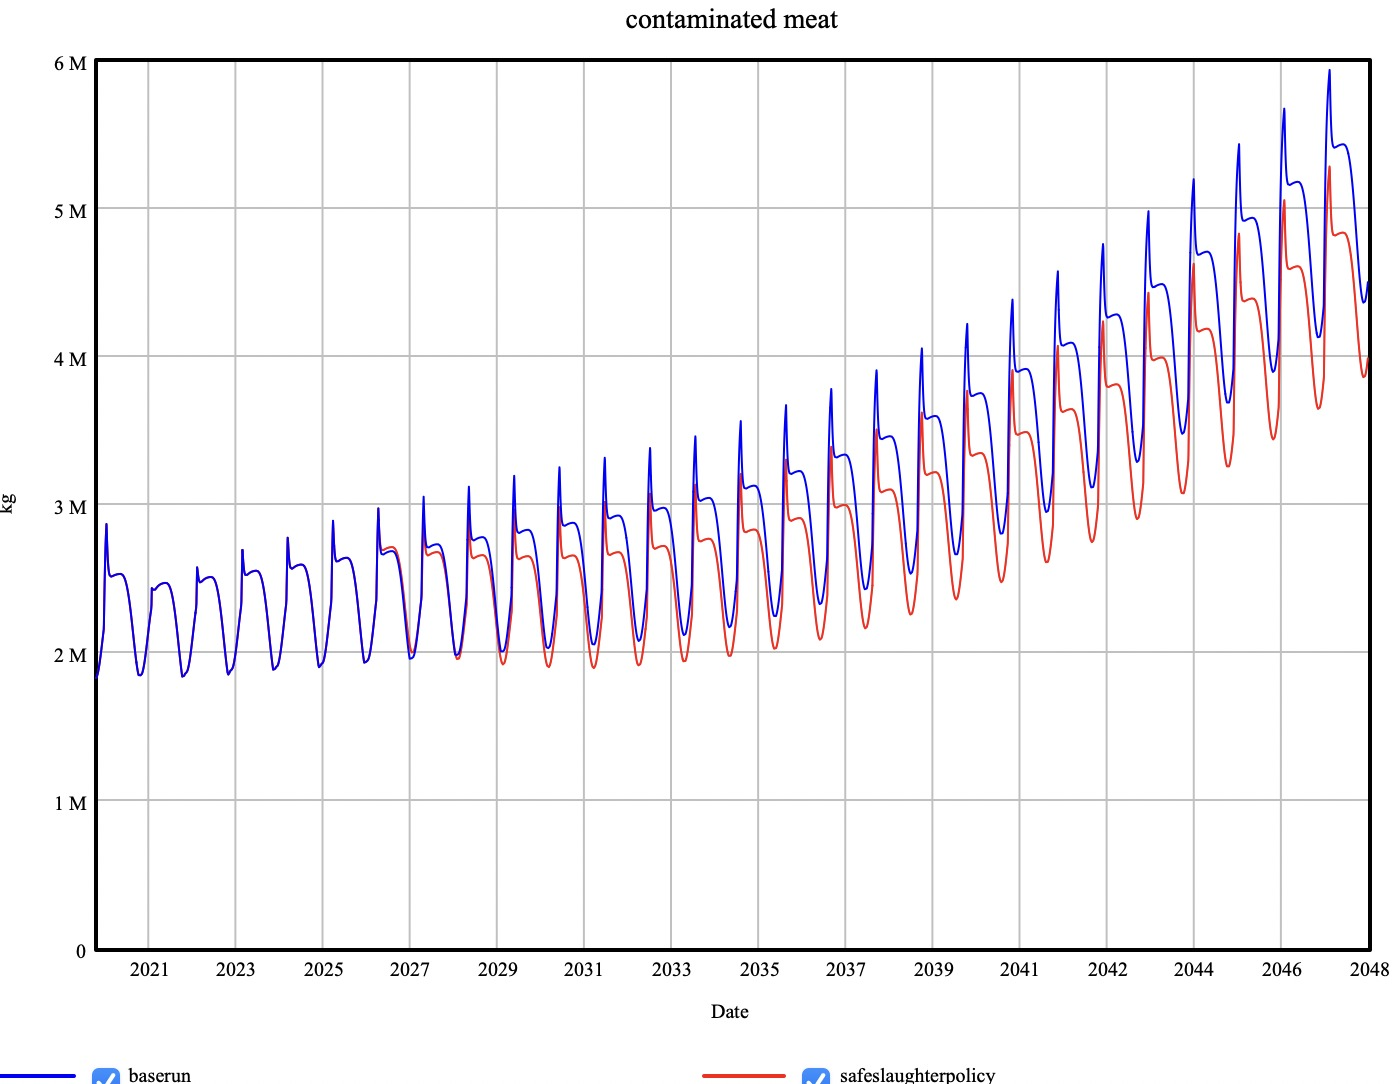
\includegraphics[width=1\textwidth]{images/p_meat.jpeg}
        \caption{Contaminated chicken meat in the Safe Slaughtering base run}
        \label{fig:p_meat}
    \end{minipage}
\end{figure} 

The model acts according to reason. It can be seen that once the food safety and handling policy goes into effect, the stock of contaminated meat decreases before slowly increases again. This shows that it has an immediate effect, which stays over time but then continues growing. 

The odd spikes in Figure \ref{fig:p_meat} are similar to the ones as explained in section \ref{s:b_base}. 

Another policy implemented was the campaign to limit human exposure to flies, dubbed the No Fly Zone. This campaign would inform the Dutch population on how to minimize attractive environments for fly propagation. This policy reduces the rate of human exposure to infectious flies by 20\%. 

\begin{figure}[h!]
    \centering
    \begin{minipage}{0.45\textwidth}
        \centering
        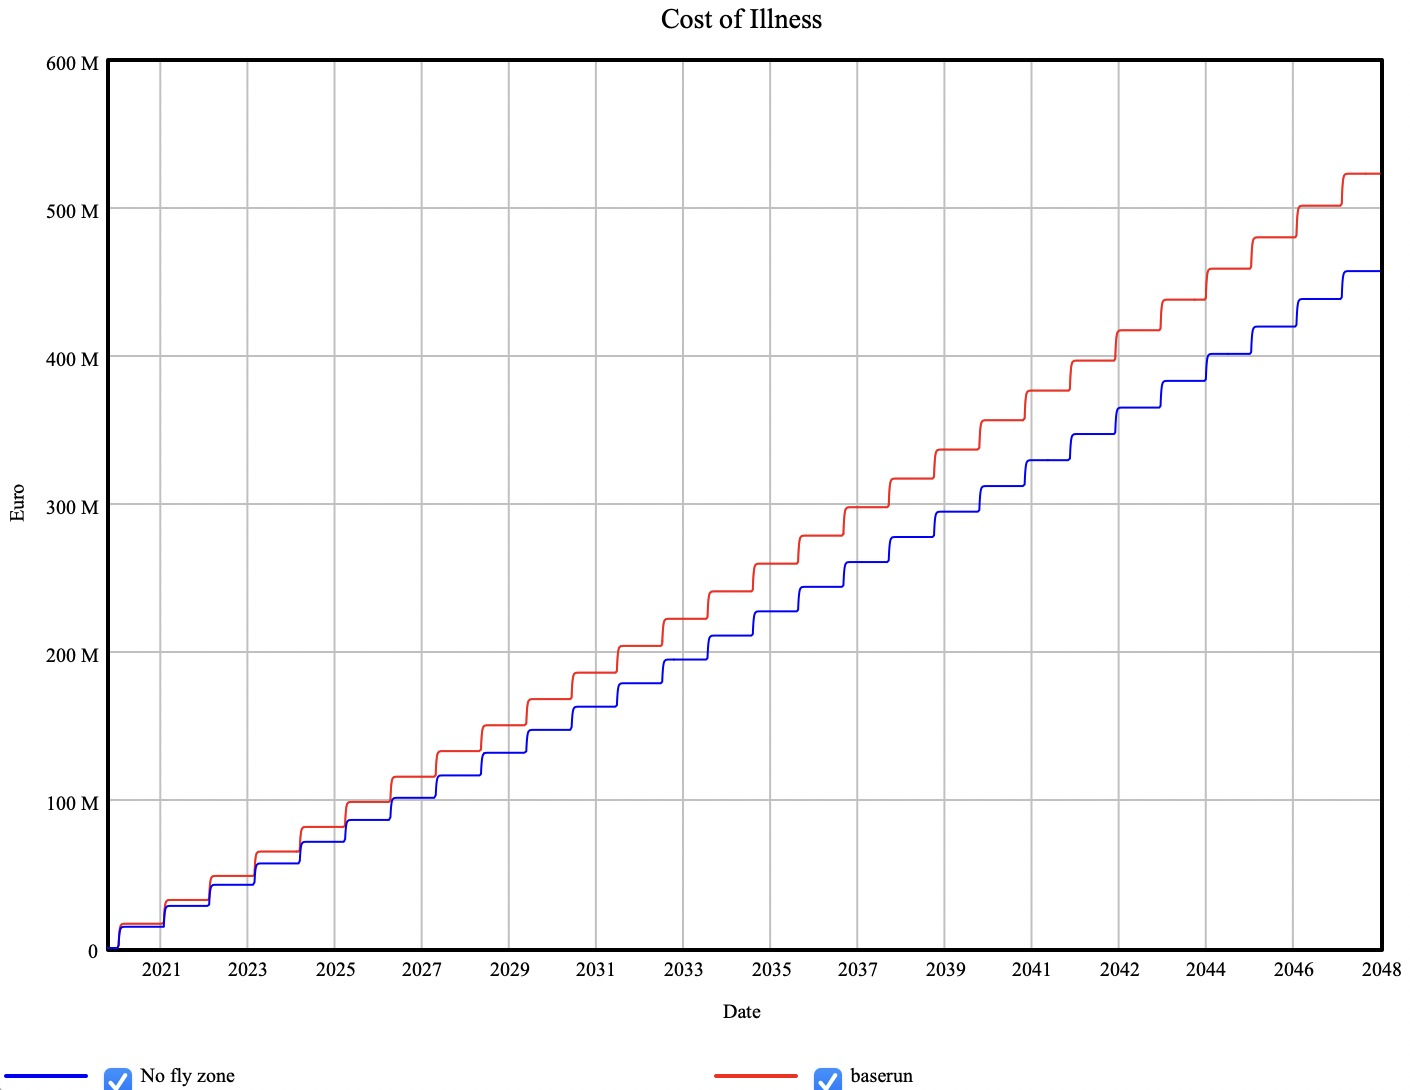
\includegraphics[width=1\textwidth]{images/p2_coi.jpeg} 
        \caption{Cost of Illness in the No Fly Zone base run}
        \label{fig:p2_coi}
    \end{minipage}\hfill
    \begin{minipage}{0.45\textwidth}
        \centering
        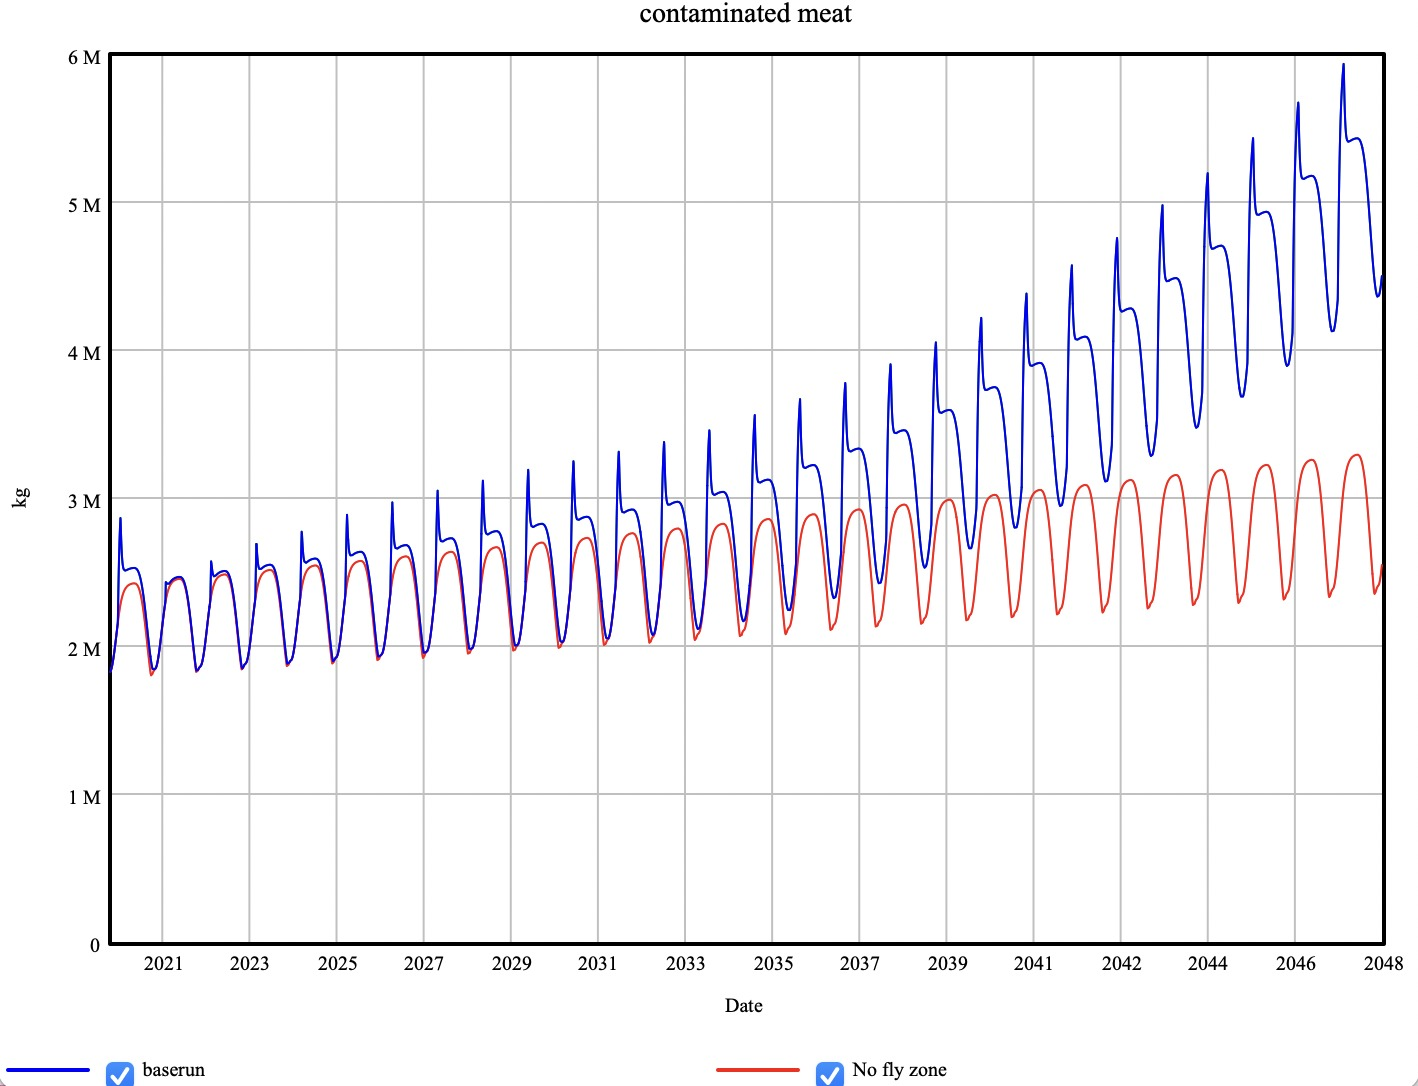
\includegraphics[width=1\textwidth]{images/p2_meat.jpeg}
        \caption{Contaminated chicken meat in the No Fly Zone base run}
        \label{fig:p2_meat}
    \end{minipage}
\end{figure} 

It can be seen in Figure \ref{fig:p2_meat} that the policy removes the strange peaks in the baserun. This is most likely due to the fact that the policy lowers the number of \textit{Campylobacter} cases, which doesn't decrease of chicken meat consumption. This means that the threshold isn't met to trigger the meat consumption behaviour while the stock of contaminated meat decreases accordingly. 

Another fly related policy which was implemented is the the Pest Control policy. This Pest Control policy entails the influence onto the fly population 

\subsubsection{Population scenarios}


\subsubsection{Climate scenarios}

\subsubsection{Public health scenarios}